\chapter{Rendre visible : quantifier les choix éthiques}
\label{chapter:modelisation}
\newrefsegment
\PEEL{Les différents choix de modélisation abordés plus haut ont une variation sur le niveau de dommage importantes, presque aussi / plus importante que d'autres facteurs souvent pris en compte (incertitude, scénario climatique).}{On utilise une analyse économétrique pour essayer de quantifier ce phénomène. }{Même si les résultats ne sont pas super forts, on voit qu'il y a une variation importante qui est issue de la variation de ces paramètres éthiques.}{Le modèle ne donne pas de vérité absolue, il sort ce qu'on y a fait entrer => les modèles sont profondément politiques, et reflètent en ce sens une certaine conception du monde.}




\chapterabstract{Ce chapitre propose une approche plus économétrique des effets de la modélisation des fonctions de dommage. On utilise le modèle WILIAM, qui pourrait devenir un modèle de référence de la commission européenne, auquel on change les fonctions de dommage. On le fait tourner avec de nombreux scénarios, pour obtenir des résultats. On réalise ensuite une étude économétrique de ces résultats, pour savoir qu'elle paramètre a le plus d'effet sur les résultats du modèle.}

\cite{errickson_equity_2021} => il peut y avoir une plus grande variation du SCC selon l'équité que selon l'incertitude climatique

Nous avons vu dans le chapitre précédent que les modèles varient dans leurs choix de représentations des dommages. De plus, ces différents choix semblent tous valables à leur manière : les phénomènes représentés sont incertains, et cette variabilité représente surtout l'incertitude qui entoure ces phénomènes. Pourtant, ce sont bien les mêmes phénomènes; il ne devrait donc pas y avoir de différence entre les modèles. Ces différences sont donc apportées exclusivement par les choix de modélisation; or, elles peuvent être importantes, et donner des conclusions radicalement différentes, donnant lieu à des interprétations opposées. La querelle entre Nordhaus et Stern, évoquée plus haut, en est un exempe éloquent. On définit ici la notion de paramètre éthique : elle désigne les paramètres qui n'ont pas vocation à représenter un phénomène physique ou social observable, mais plutot à représenter une valeur morale. Le taux d'actualisation, par exemple, entre tout à fait dans cette définition. En effet, il représente l'importance accordée à l'équité inter-générationnelle. bien qu'il y ait eu des tentatives d'observer empiriquement cette valeur, notamment en s'intéressant au taux de préférence pure pour le présent dans les prêts de long terme, il semble difficile de penser que cette valeur soit valable a plus long terme ou dans d'autres contexte. Plutot, il apparait que ce paramètre reflète un système normatif, et relève de ce fait plutot du choix moral que du choix technique. Se pose alors la question suivante : quelle part de la variation du niveau total de dommage est-elle expliquée par ces paramètres éthiques. Dans cette partie, on développe un protocole expérimental qui vise à mesurer le niveau de dommage produit par différents modèles, différentes fonctions de dommages et surtout différents niveau pour ces paramètres éthiques. On régresse ensuite les données obtenues pour mesurer quantitativement la part de la variation qui est expliquée par ces fameux paramètres. 

\section{Cadre conceptuel}

Le cadre conceptuel général de cette expérience est celui de la modélisation intégré. Il s'inscrit en cela dans la lignée des réflexions développées dans le chapitre \ref{chapter:introduction}. Il semble néanmoins nécessaire de préciser quelques points. \\

D'abord, le choix du modèle. Pour réaliser cette expérience, nous avons choisi d'utiliser le modèle WILIAM, pour plusieurs raisons. 

\paragraph{Modèle Open-source}WILIAM est un modèle Open-Source, ce qui signifie que l'ensemble du code source est disponible en ligne, avec une licence permettant une utilisation, diffusion et modification du programme sans limites. C'est nécessaire puisqu'on a ainsi accès à tous le code source, ce qui permet de travailler sur une base solide; on peut également le modifier librement, ce qui est au coeur de l'expérience; enfin, on peut le diffuser librement aussi, ce qui est fait à travers le dépôt GitHub et le blog. Par ailleurs, bien que ce ne soit pas en soi une garantie de qualité, l'utilisation de l'open source permet d'améliorer la robustesse et la transparence des modèles, puisque chacun peut voir les hypothèses, proposer des modifications, et corriger des erreurs. 

\paragraph{Application aux politiques publiques} WILIAM est issu du projet LOCOMOTION, financé par la Commission Européenne. Il répond à une demande de celle-ci de s'équiper d'un nouveau modèle. Ainsi, WILIAM est un modèle qui vise à répondre à des questions de politique publique. 

\paragraph{Modèle complexe} WILIAM est un modèle particulièrement complexe : il compte près de 4000 variables. Cela le rend particulièrement vulnérable aux problématiques de transparence et de complexité excessive que nous développerons plus tard. Néanmoins, cela nous permet d'avoir un modèle le plus comple possible. Cela permet d'intégrer les fonctions de dommage facilement, car les variables sont déjà existantes. 

\paragraph{Modèle de simulation} WILIAM est un modèle de simulation. Cette caractéristique est importante car elle permet de voir les valeurs de chaque paramètre à tout moment, mais aussi de représenter des paramètres non-monétaires. De plus, ça le rend moins sensible aux critiques de normativité inhérente aux modèles d'optimisation \ref{}. 

\section{Méthode}

\begin{methodbox}[Modélisation des fonctions de dommage dans WILIAM]

Pour modéliser les fonctions de dommage dans WILIAM, on commence par créer un nouveau repo sur github, dans lequel on télécharge le code source de WILIAM. On s'assure que tout est fonctionnel, et que le modèle tourne bien. La visualisation du modèle se fait grâce au logiciel VENSIM. \\

On rassemble les sources de données disponibles des modèles : code source, documentation et / ou publications qui y font référence. Ces sources n'offrent pas le même niveau d'information. Par exemple, les modèles dont on ne trouve pas le code source mais uniquement des publications sont plus difficiles à modéliser car il manque souvent des informations cruciales, telles que les valeurs obtenues pour les paramètres. \\

Une fois la définition de la fonction identifiée, on les modélise à l'aide de l'interface graphique du logiciel VENSIM. On sauvegarde régulièrement, en réalisant des \textit{commit} sur github pour garder une trace de la progression.
    
\end{methodbox}

\begin{methodbox}[Conversion des paramètres selon les bonnes zones géographiques]

    Le modèle WILIAM comporte 35 régions. En revanche, les autres modèles n'ont pas nécessairement le même découpage géographique. Deux cas se distinguent : soit le modèle est agrégé au niveau mondial; on peut alors utiliser les fonctions de dommage région par région, sans besoin de les changer. Soit le modèle possède des régions, et il faut alors convertir les régions du modèle A en régions de WILIAM pour avoir la bonne paramètrisation. Ce deuxième cas de figure est particulièrement vrai dans le cas du modèle FUND, qui a des régions très différentes de celles de WILIAM, et qui repose beaucoup sur de la paramétrisation. Il faut donc convertir les paramètres des régions de FUND en régions de WILIAM. 

    Par ailleurs, il est à noter que si la documentation de FUND est très complète et accessible en ligne, les tables de paramètre ne sont pas disponible dans un format facilement lisible tel que CSV. La méthode retenue a été de lire la page de la documentation (en markdown), et de la découper table par table puis valeur par valeur à l'aide d'un script python, qui permet ensuite d'enregistrer ces données dans un format lisible par VENSIM. Ces opérations sont longues et peuvent être source de nombreuses erreurs. Ainsi, le non-partage des données dans un format standard est un vrai frein à la reproductibilité. \\
    
    On utilise alors un script Python qui désagrège les zones de FUND en pays, et qui associe à chaque pays sa zone dans WILIAM. 
    
\end{methodbox}

La plupart des fonctions de dommage dépendent du niveau de revenu par habitant, de plusieurs manières. Le premier cas de figure est qu'elles donnent un niveau de dommage qui est exprimé en proportion du PIB. On a alors un niveau de dommage absolu qui est plus grand dans les régions plus riches, puisque le PIB est lui-même plus grand. Ce point est essentiel, en particulier dans les modèles d'optimisation. En effet, ces modèles cherchant à trouver la solution la moins couteuse, ils vont être beaucoup plus sensibles aux dommages dans les pays ayant un PIB plus important que dans les pays ayant un niveau de revenu plus faible. \emph{De facto}, ils vont chercher à minimiser les dommages dans les pays les plus riches, quitte à augmenter les dommages dans les pays les plus pauvres. \\

La deuxième manière est que la fonction de dommage intègre directement le niveau de revenu dans le calcul du niveau de dommage. Selon le signe de l'équation, cette méthode peut renforcer les effets dans les pays les plus pauvres, ou au contraire les augmenter. 

On peut finalement citer une technique permettant de monétiser des impacts non-monétaires, tels que des morts ou des années d'invalidité. La technique utilisée est assez classique en économie : il s'agit de calculer la valeur d'une vie statistique, ou \emph{value of a statistical life} (VSL). Cette méthode part de l'hypothèse que la valeur de la vie dans un lieu donnée correspond à un certain multiple du niveau de revenu par habitant dans ce lieu. On peut prendre en exemple la VSL du modèle FUND, qui prend la forme suivante : 

\begin{equation}
    VSL_{t, r} = \alpha (\frac{y_{t,r}}{y_0})^\epsilon
\end{equation}
où $t$ désigne l'année, $r$ désigne la région, $\alpha$ et $\epsilon$ des paramètres permettant de calibrer la fonction, $y_{t,r}$ le revenu par habitant dans la région $t$ à l'instant $r$, et $y_0$ un revenu de référence.  \\

Ce choix de modélisation pose de nombreuses questions. 
D'abord, d'un point de vue pragmatique. Les pays les plus pauvres sont susceptibles d'être les pays les plus impactés par le changement climatique, d'une part par une exposition plus grande à des phénomènes extremes, et d'autre part par une situation de pauvreté préexistante qui fragilise la résilience. 
Ensuite, pour des raisons morales. Le principe de responsabilité commune mais différenciée sur le changement climatique, qui préside le régime climatique depuis sa formation, instaure une distinction claire entre les pays des Nords, qui ont bénéficié de l'émission de carbone pendant des décennies pour leur développement, et les pays des Suds, dont le poids historique est relativement limité. On pourrait penser qu'il est souhaitable de pénaliser grandement les impacts du changement climatique dans les pays des Suds, du fait de cette responsabilité moindre. 
Enfin,  on peut aussi envisager une perspective de justice sociale pour traiter de ce sujet. On peut par exemple imaginer que les dommages sur les plus pauvres, touchant des populations déjà fragiles, sont particulièrement impactants. Il pourrait être dès lors notre responsabilité de limiter ces impacts, à la manière du Maximin de Rawls. 

Notre propos ici n'est pas de défendre l'une ou l'autre de ces positions. Chacune défend un objectif et un système normatif différent. Elles ont toutes leurs arguments et leurs travers, et il n'est pas question d'affirmer que l'une d'elle est la seule manière possible de concevoir le problème. Il s'agit même plutot de l'inverse : montrer qu'une multitude de choix de modélisation existent, et que leurs implications sont radicalement différentes. 

En revanche, nous argumentons qu'il y a nécessairement, dans les pratiques de modélisation, le choix de l'une ou l'autre de ces conceptions.  Nous cherchons dès lors à comprendre les effets de ce choix sur le niveau de sortie du modèle, en appliquant un coefficient éthique (voir encadré méthodologique) en sortie des fonctions de dommage. Le rôle de ce coefficient est précisément de  rendre visible l'existence de ce choix, et de permettre aux utilisateurs de varier les paramètres. 

\begin{methodbox}[Définition d'un coefficient éthique]
Nous observons la forme de la valeur d'une vie statistique, développée dans FUND. Cette expression est une bonne référence, car : 

\begin{itemize}
    \item il s'agit d'une pratique courante
    \item elle représente un phénomène dont on pourrait penser qu'il ait la même valeur partout (en l'occurence, la mort)
\end{itemize}

Cette expression permet de comparer un même phénomène (la mort), dans des contextes où le revenu est différent. Elle est donc adaptée pour représenter un même phénomène (un niveau de dommage, au sens physique) dans un système de comptabilité différent (en l'occurence monétaire). 

Nous l'adaptons ainsi : 

\begin{itemize}
    \item les variations du coefficient $\alpha$ permettent de faire varier le sens et l'intensité de la relation entre niveau de revenu et niveau de dommage comptabilisé
    \item les variations de $y_0$ permettent de faire varier la limite entre les pays considérés comme riches et les pays considérés comme pauvres
    \item les variations de $\epsilon$ permettent de faire varier la convexité de la relation, c'est à dire à quelle point les valeurs pour les différents pays vont être différentes. 
\end{itemize}

\vspace{2cm}

\centering
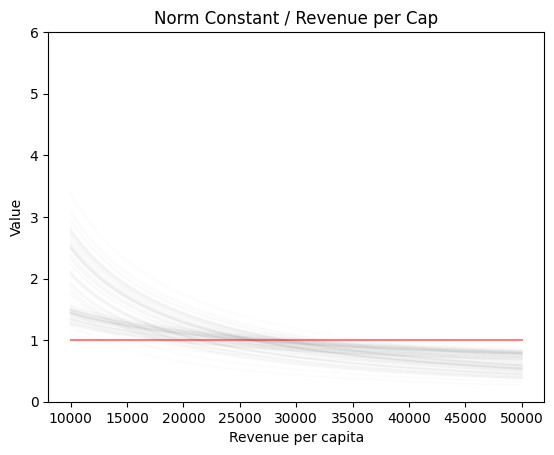
\includegraphics[width=0.75\linewidth]{figures/coef.png}

\end{methodbox}
\begin{methodbox}[Execution des différents runs]

    
    
\end{methodbox}

\begin{methodbox}
On utilise ici le modèle WILIAM. Il s'agit d'un modèle open source, donc il est assez facile de le répliquer, modifier et distribuer. Le code source est disponible sur Github. On réalise une fork du code source, c'est-à-dire une branche de code. Notre branche de code devient un projet autonome sur lequel on peut travailler de manière semi-indépendante du projet. En effet, les modifications du projet WILIAM ou celles réalisées ici ne s'affecteront pas, à moins que l'on push notre code vers le code principal, ou que l'on pull les nouvelles modifications du code principal vers notre branche. Ces deux opérations peuvent se faire sous supervision, pour s'assurer que l'on n'interagit pas avec différentes parties de notre code, ce qui risquerait de fausser nos résultats. \blog{https://damage-functions-modeling.readthedocs.io/en/latest/3_notebooks/spatial_temporal_equity.html} \\

Dans cette branche, on modifie le code pour qu'il représente les fonctions de dommage. On modélise ainsi plusieurs formes de fonctions de dommage, issues de la revue de littérature évoquée plus haut. On fait tourner le modèle avec ces différentes fonctions de dommage, et en faisant varier aléatoirement les différents paramètres : taux d'actualisation, les différents paramètres qui entrent en compte dans le modèle. \\

On récupère les résultats et on procéde à des analyses économétriques sur les résultats pour voir quels sont les paramètres qui ont le plus influencé les résultats. La largeur de la page est \the\textwidth. En centimètres, cela donne \uselengthunit{cm}\printlength{\textwidth}.

\end{methodbox}

\begin{figure}
    \centering
    \begin{overpic}[width=\linewidth,grid,tics=10]{illustrations/methodo_econometrie.png}
        \put(10, 90){WILIAM}
        \put(50,70){\Huge $E=mc^2$} % Texte au centre de l'image
        \put(10,20){\color{red}\huge Important} % Texte en bas à gauche
    \end{overpic}
    %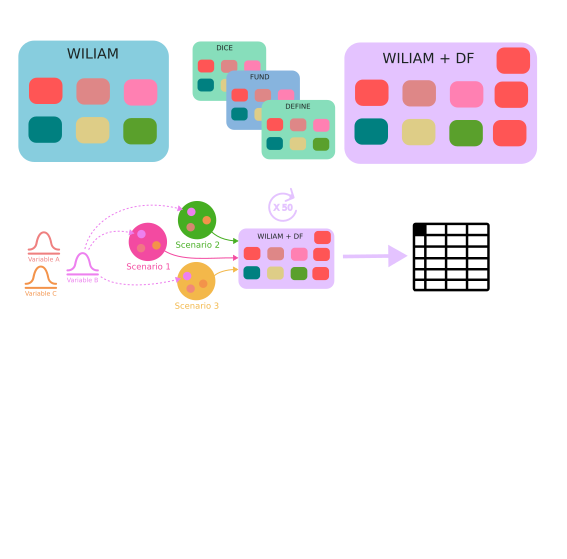
\includegraphics[width=0.9\textwidth]{illustrations/methodo_econometrie.png}
    \legende{Méthodologie de la comparaison des modèles. (SVG)}{On utilise le modèle open-source WILIAM. Celui ci est composé de différents modules, dont un module représentant les dommages (représenté ici en rouge). On identifié les fonctions de dommage d'autres modèles (DICE, FUND et DEFINE). On les isole, et on les implémente dans le modèle WILIAM. On a alors un nouveau modèle, qui contient simultanément plusieurs manières de représenter les dommages. On connait la distribution de certains paramètres, et on cherche à voir l'effet de cette variation sur les résultats du modèle. On réalise des scénarios, qui sont des combinaisons de tirage aléatoire des variables. Le modèle est executé avec chaque scénario, de nombreuses fois. Tous ces \textit{runs} forment une grande base de donnée, sur laquelle on va réaliser une étude économétrique. }
    \label{fig:methodo-simu}
\end{figure}

\section{Limites et contraintes}

Plusieurs limitations doivent être soulignées. 

\paragraph{Transposition dans un autre modèle} D'abord, on utilise les fonctions de dommage de différents modèles dans le modèle WILIAM. Cela permet d'avoir les même conditions pour toutes les fonctions de dommage. Ceci étant dit, les fonctions ne sont plus dans leur milieu d'origine. Ceci pose deux problème. D'abord, les fonctions peuvent avoir été calibrées pour fonctionner correctement dans certaines conditions de fonctionnement de température, et pas au delà; et ces conditions peuvent ne pas être atteinte dans WILIAM. Cela est notamment vrai pour toutes les variables qui nécessitent une calibration, par exemple celles où la population entre en jeux. Une population différente peut aboutir à une fonction de dommage qui est différente. Ensuite, il y a un grand risque d'erreur de transcription. En effet, les variables peuvent avoir les mêmes noms mais ne pas désigner la même chose précisement ou ne pas être calculée de la même manière; ou encore, la documentation d'origine peut ne pas être claire sur les caractéristiques précises d'une variable (notamment, le niveau de désagrégation). On peut néanmoins considérer que ce n'est pas une limitation très forte. En effet, nous nous intéressons ici à la \emph{relation} entre les hypothèses et le niveau de dommage, et pas au niveau de dommage \emph{en soi}. Ainsi, une mauvaise calibration risque de donner des valeurs trop faibles ou trop élèvées, mais n'a pas d'effet sur la relation en soi. Par ailleurs, ces fonctions sont justement présentées comme des relations liant les phénomènes climatiques à un niveau de dommage. Si changer de modèle affecte grandement la validité de la relation, alors on peut interroger la validité de la relation dans son ensemnle. 

\paragraph{Collinéarité} Le problème majeur de cette technique est que les données analysées ont été produites dans la perspective de cette analyse. Ainsi, il est possible que le résultat de l'analyse de reflète que les hypothèses et les variations qui ont été volontairement ajoutées au modèle. En particulier, le niveau de dommage dépend beaucoup de la valeur du coefficient d'éthique spatial, qui est lui même construit pour l'expérience. 






\begin{figure}
    \centering
    
\definecolor{c87cdde}{RGB}{135,205,222}
\definecolor{c1c2422}{RGB}{28,36,34}
\definecolor{teal}{RGB}{0,128,128}
\definecolor{cdecd87}{RGB}{222,205,135}
\definecolor{c5aa02c}{RGB}{90,160,44}
\definecolor{cff5555}{RGB}{255,85,85}
\definecolor{cde8787}{RGB}{222,135,135}
\definecolor{cff80b2}{RGB}{255,128,178}
\definecolor{ce4c3ff}{RGB}{228,195,255}
\definecolor{c87debb}{RGB}{135,222,187}
\definecolor{c616161}{RGB}{97,97,97}
\definecolor{c87b4de}{RGB}{135,180,222}
\definecolor{cef8080}{RGB}{239,128,128}
\definecolor{ced80ef}{RGB}{237,128,239}
\definecolor{cf3934a}{RGB}{243,147,74}
\definecolor{cf34aa1}{RGB}{243,74,161}
\definecolor{c46ae22}{RGB}{70,174,34}
\definecolor{cf3b84a}{RGB}{243,184,74}
\definecolor{c82d71f}{RGB}{130,215,31}
\definecolor{lightcoral}{RGB}{240,128,128}
\definecolor{c949494}{RGB}{148,148,148}
\definecolor{cff7b88}{RGB}{255,123,136}
\definecolor{cafbbd0}{RGB}{175,187,208}
\definecolor{ca1a8bb}{RGB}{161,168,187}
\definecolor{cd1d9e9}{RGB}{209,217,233}
\definecolor{c5a5a5a}{RGB}{90,90,90}
\definecolor{cf34a7d}{RGB}{243,74,125}


\def \globalscale {1.000000}
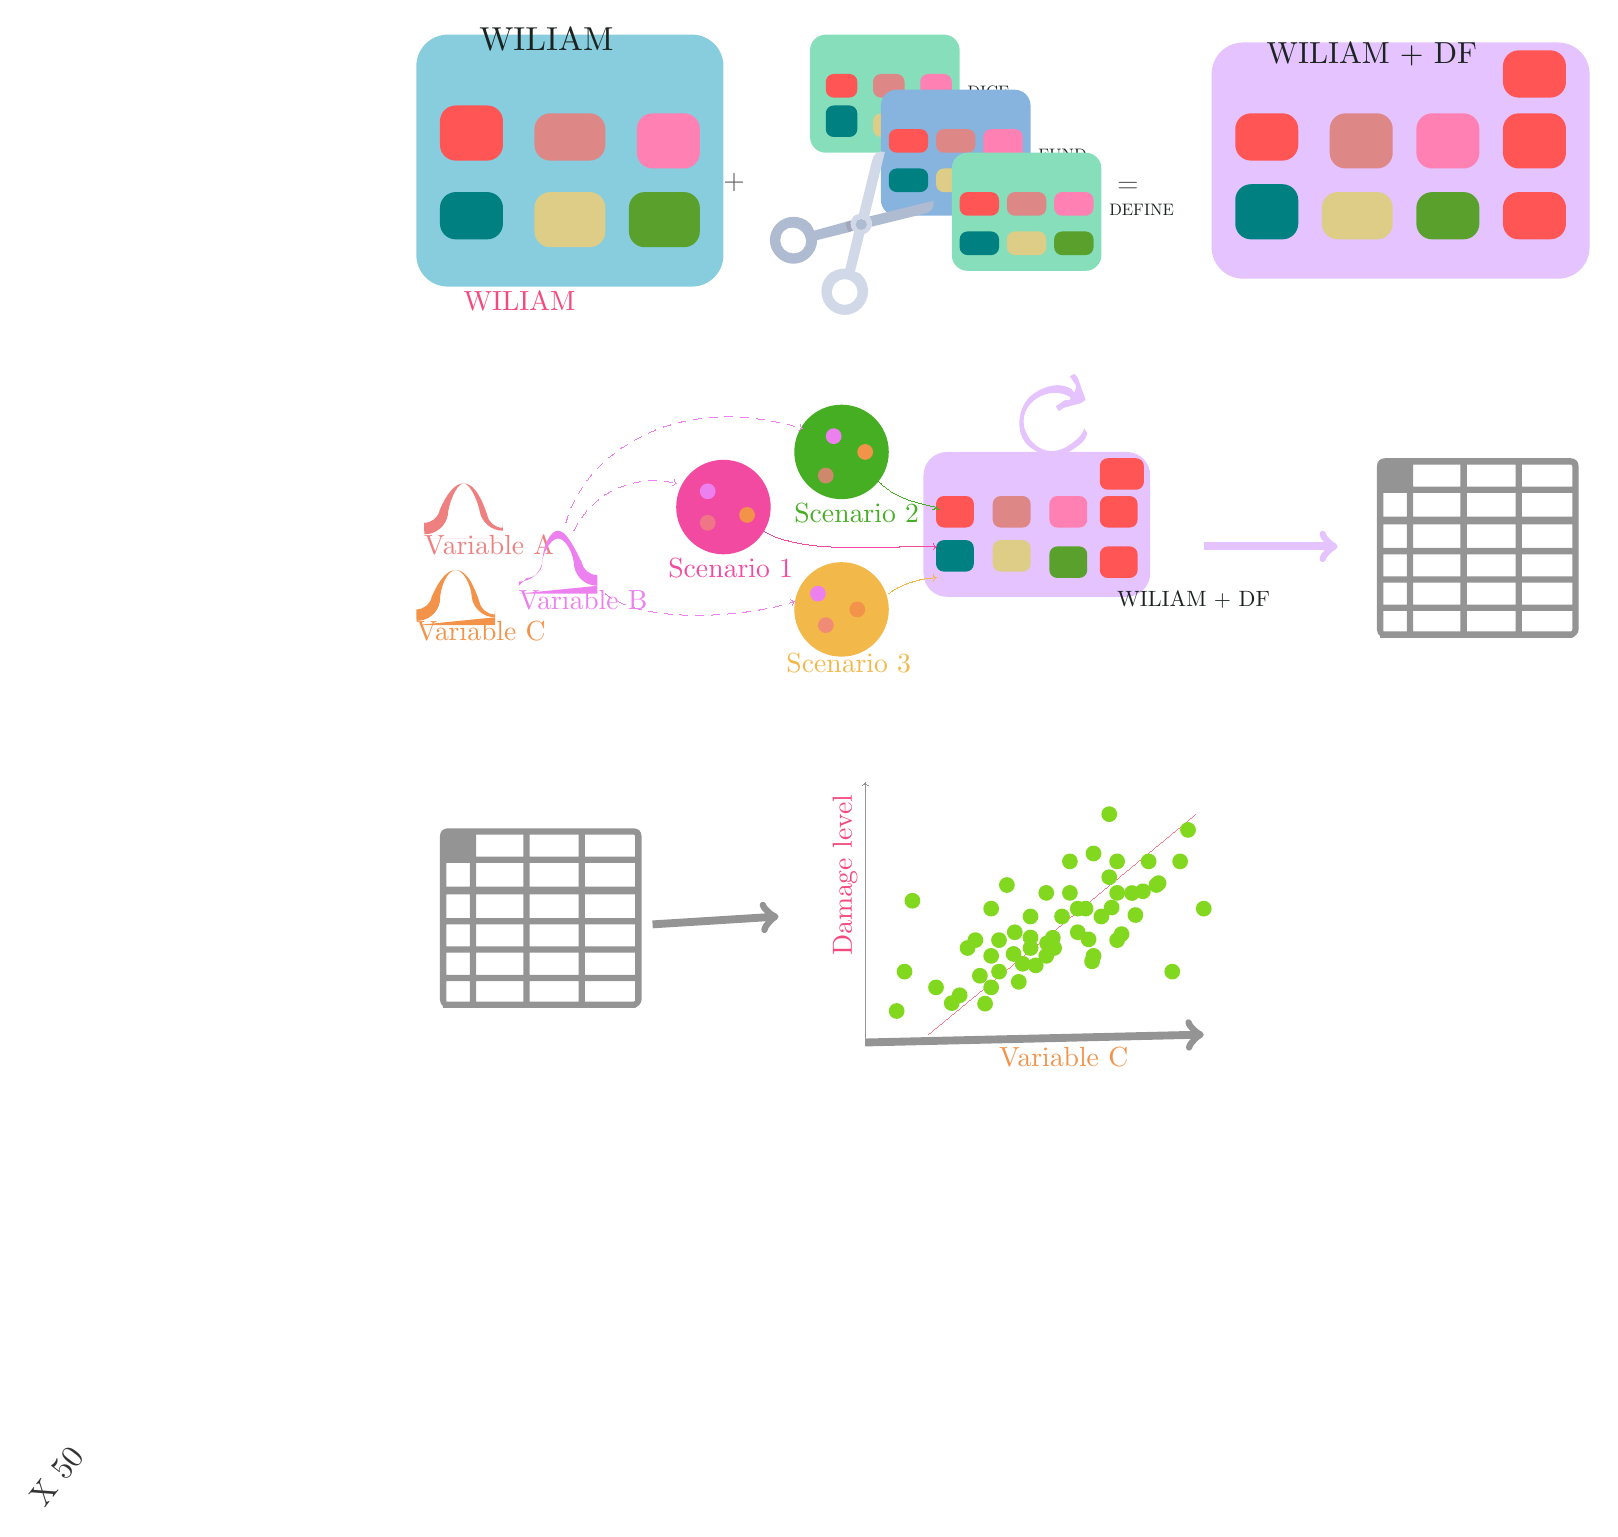
\begin{tikzpicture}[y=1cm, x=1cm, yscale=\globalscale,xscale=\globalscale, every node/.append style={scale=\globalscale}, inner sep=0pt, outer sep=0pt]
  \path[fill=c87cdde,line width=0.0cm,rounded corners=0.4cm] (0.1, 14.7) 
  rectangle (4.0, 11.5);



  \node[text=c1c2422,cm={ 1.2,-0.0,-0.0,1.2,(-2.1, 1.1)},anchor=south west] 
  (text1) at (3.0, 13.4){WILIAM};



  \node[text=c1c2422,anchor=south west] (text2) at (3.0, 12.3){};



  \path[fill=teal,line width=0.0cm,rounded corners=0.2cm] (0.4, 12.7) rectangle 
  (1.2, 12.1);



  \path[fill=cdecd87,line width=0.0cm,rounded corners=0.2cm] (1.6, 12.7) 
  rectangle (2.5, 12.0);



  \path[fill=c5aa02c,line width=0.0cm,rounded corners=0.2cm] (2.8, 12.7) 
  rectangle (3.7, 12.0);



  \path[fill=cff5555,line width=0.0cm,rounded corners=0.2cm] (0.4, 13.8) 
  rectangle (1.2, 13.1);



  \path[fill=cde8787,line width=0.0cm,rounded corners=0.2cm] (1.6, 13.7) 
  rectangle (2.5, 13.1);



  \path[fill=cff80b2,line width=0.0cm,rounded corners=0.2cm] (2.9, 13.7) 
  rectangle (3.7, 13.0);



  \path[fill=ce4c3ff,line width=0.0cm,rounded corners=0.4cm] (10.2, 14.6) 
  rectangle (15.0, 11.6);



  \node[text=c1c2422,cm={ 1.1,-0.0,-0.0,1.1,(7.9, 0.9)},anchor=south west] 
  (text1-1) at (3.0, 13.4){WILIAM + DF};



  \path[fill=teal,line width=0.0cm,rounded corners=0.2cm] (10.5, 12.8) rectangle
   (11.3, 12.1);



  \path[fill=cdecd87,line width=0.0cm,rounded corners=0.2cm] (11.6, 12.7) 
  rectangle (12.5, 12.1);



  \path[fill=c5aa02c,line width=0.0cm,rounded corners=0.2cm] (12.8, 12.7) 
  rectangle (13.6, 12.1);



  \path[fill=cff5555,line width=0.0cm,rounded corners=0.2cm] (10.5, 13.7) 
  rectangle (11.3, 13.1);



  \path[fill=cde8787,line width=0.0cm,rounded corners=0.2cm] (11.7, 13.7) 
  rectangle (12.5, 13.0);



  \path[fill=cff80b2,line width=0.0cm,rounded corners=0.2cm] (12.8, 13.7) 
  rectangle (13.6, 13.0);



  \path[fill=c87debb,line width=0.0cm,rounded corners=0.2cm] (5.1, 14.7) 
  rectangle (7.0, 13.2);



  \node[text=c1c2422,cm={ 0.6,-0.0,-0.0,0.6,(4.1, 0.5)},anchor=south west] 
  (text1-8) at (3.0, 13.4){DICE};



  \path[fill=teal,line width=0.0cm,rounded corners=0.1cm] (5.3, 13.8) rectangle 
  (5.7, 13.4);



  \path[fill=cdecd87,line width=0.0cm,rounded corners=0.1cm] (5.9, 13.7) 
  rectangle (6.3, 13.4);



  \path[fill=c5aa02c,line width=0.0cm,rounded corners=0.1cm] (6.5, 13.7) 
  rectangle (6.9, 13.4);



  \path[fill=cff5555,line width=0.0cm,rounded corners=0.1cm] (5.3, 14.2) 
  rectangle (5.7, 13.9);



  \path[draw=c616161,line width=0.0cm,dash pattern=on 0.0cm off 0.0cm,rounded 
  corners=0.1cm] (5.2, 14.3) rectangle (5.7, 13.9);



  \path[fill=cde8787,line width=0.0cm,rounded corners=0.1cm] (5.9, 14.2) 
  rectangle (6.3, 13.9);



  \path[fill=cff80b2,line width=0.0cm,rounded corners=0.1cm] (6.5, 14.2) 
  rectangle (6.9, 13.9);



  \path[fill=c87b4de,line width=0.0cm,rounded corners=0.2cm] (6.0, 14.0) 
  rectangle (7.9, 12.4);



  \node[text=c1c2422,cm={ 0.6,-0.0,-0.0,0.6,(5.0, -0.3)},anchor=south west] 
  (text1-8-2) at (3.0, 13.4){FUND};



  \path[fill=teal,line width=0.0cm,rounded corners=0.1cm] (6.1, 13.0) rectangle 
  (6.6, 12.7);



  \path[fill=cdecd87,line width=0.0cm,rounded corners=0.1cm] (6.7, 13.0) 
  rectangle (7.2, 12.7);



  \path[fill=c5aa02c,line width=0.0cm,rounded corners=0.1cm] (7.3, 13.0) 
  rectangle (7.7, 12.7);



  \path[fill=cff5555,line width=0.0cm,rounded corners=0.1cm] (6.1, 13.5) 
  rectangle (6.6, 13.2);



  \path[fill=cde8787,line width=0.0cm,rounded corners=0.1cm] (6.7, 13.5) 
  rectangle (7.2, 13.2);



  \path[fill=cff80b2,line width=0.0cm,rounded corners=0.1cm] (7.3, 13.5) 
  rectangle (7.8, 13.1);



  \path[fill=c87debb,line width=0.0cm,rounded corners=0.2cm] (6.9, 13.2) 
  rectangle (8.8, 11.7);



  \node[text=c1c2422,cm={ 0.6,-0.0,-0.0,0.6,(5.9, -1.0)},anchor=south west] 
  (text1-8-4) at (3.0, 13.4){DEFINE};



  \path[fill=teal,line width=0.0cm,rounded corners=0.1cm] (7.0, 12.2) rectangle 
  (7.5, 11.9);



  \path[fill=cdecd87,line width=0.0cm,rounded corners=0.1cm] (7.6, 12.2) 
  rectangle (8.1, 11.9);



  \path[fill=c5aa02c,line width=0.0cm,rounded corners=0.1cm] (8.2, 12.2) 
  rectangle (8.7, 11.9);



  \path[fill=cff5555,line width=0.0cm,rounded corners=0.1cm] (7.0, 12.7) 
  rectangle (7.5, 12.4);



  \path[fill=cde8787,line width=0.0cm,rounded corners=0.1cm] (7.6, 12.7) 
  rectangle (8.1, 12.4);



  \path[fill=cff80b2,line width=0.0cm,rounded corners=0.1cm] (8.2, 12.7) 
  rectangle (8.7, 12.4);



  \path[fill=cff5555,line width=0.0cm,rounded corners=0.2cm] (13.9, 14.5) 
  rectangle (14.7, 13.9);



  \path[fill=cff5555,line width=0.0cm,rounded corners=0.2cm] (13.9, 13.7) 
  rectangle (14.7, 13.0);



  \path[fill=cff5555,line width=0.0cm,rounded corners=0.2cm] (13.9, 12.7) 
  rectangle (14.7, 12.1);



  \begin{scope}[cm={ 0.8,-0.0,-0.0,0.8,(-0.9, 4.2)}]
    \path[fill=ce4c3ff,line width=0.0cm,rounded corners=0.3cm] (9.3, 6.5) 
  rectangle (12.9, 4.2);



    \node[text=c1c2422,cm={ 0.8,-0.0,-0.0,0.8,(7.5, -7.5)},anchor=south west] 
  (text1-1-8) at (3.0, 13.4){WILIAM + DF};



    \path[fill=teal,line width=0.0cm,rounded corners=0.1cm] (9.5, 5.1) rectangle
   (10.1, 4.6);



    \path[fill=cdecd87,line width=0.0cm,rounded corners=0.1cm] (10.4, 5.1) 
  rectangle (11.0, 4.6);



    \path[fill=c5aa02c,line width=0.0cm,rounded corners=0.1cm] (11.3, 5.0) 
  rectangle (11.9, 4.5);



    \path[fill=cff5555,line width=0.0cm,rounded corners=0.1cm] (9.5, 5.8) 
  rectangle (10.1, 5.3);



    \path[fill=cde8787,line width=0.0cm,rounded corners=0.1cm] (10.4, 5.8) 
  rectangle (11.0, 5.3);



    \path[fill=cff80b2,line width=0.0cm,rounded corners=0.1cm] (11.3, 5.8) 
  rectangle (11.9, 5.3);



    \path[fill=cff5555,line width=0.0cm,rounded corners=0.1cm] (12.1, 6.4) 
  rectangle (12.8, 5.9);



    \path[fill=cff5555,line width=0.0cm,rounded corners=0.1cm] (12.1, 5.8) 
  rectangle (12.7, 5.3);



    \path[fill=cff5555,line width=0.0cm,rounded corners=0.1cm] (12.1, 5.0) 
  rectangle (12.7, 4.5);



  \end{scope}
  \path[fill=cef8080,line width=0.0cm] (1.2, 8.3) -- (0.2, 
  8.3)arc(90.0:270.0:0.0) -- (1.2, 8.3)arc(-90.0:90.0:0.0) -- cycle;



  \path[fill=cef8080,line width=0.0cm] (1.2, 8.4) -- (1.2, 
  8.4)arc(89.9:169.8:0.3 and -0.3).. controls (0.9, 8.7) and (0.8, 9.0) .. (0.7,
   9.0).. controls (0.6, 9.0) and (0.5, 8.7) .. (0.5, 8.6)arc(10.4:90.2:0.3 and 
  -0.3) -- (0.2, 8.4)arc(89.9:270.1:0.0) -- (0.2, 8.5)arc(90.0:10.7:0.2 and 
  -0.2).. controls (0.5, 8.9) and (0.6, 9.0) .. (0.7, 9.0).. controls (0.8, 9.0)
   and (0.9, 8.9) .. (1.0, 8.6)arc(169.5:90.1:0.2 and -0.2) -- (1.2, 
  8.5)arc(-89.89999999999998:89.9:0.0) -- cycle;



  \path[fill=black,fill opacity=0.0,line width=0.0cm] (0.1, 9.2) rectangle (1.3,
   8.1);



  \node[text=cef8080,line width=0.0cm,anchor=south west] (text4) at (0.2, 
  8.1){Variable A};



  \path[fill=ced80ef,line width=0.0cm] (2.4, 7.6) -- (1.4, 
  7.6)arc(89.8:270.2:0.0) -- (2.4, 7.7)arc(-90.19999999999999:90.2:0.0) -- cycle;



  \path[fill=ced80ef,line width=0.0cm] (2.4, 7.7) -- (2.4, 
  7.7)arc(89.9:169.8:0.3 and -0.3).. controls (2.1, 8.1) and (2.0, 8.3) .. (1.9,
   8.3).. controls (1.8, 8.3) and (1.7, 8.1) .. (1.7, 8.0)arc(10.4:90.2:0.3 and 
  -0.3) -- (1.4, 7.7)arc(90.0:270.0:0.0) -- (1.5, 7.8)arc(90.0:10.7:0.2 and 
  -0.2).. controls (1.7, 8.2) and (1.8, 8.4) .. (1.9, 8.4).. controls (2.0, 8.4)
   and (2.1, 8.2) .. (2.2, 8.0)arc(169.5:90.1:0.2 and -0.2) -- (2.4, 
  7.8)arc(-89.89999999999998:89.9:0.0) -- cycle;



  \node[text=ced80ef,line width=0.0cm,anchor=south west] (text4-4) at (1.4, 
  7.4){Variable B};



  \path[fill=cf3934a,line width=0.0cm] (1.1, 7.2) -- (0.1, 
  7.2)arc(89.9:270.1:0.0) -- (1.1, 7.3)arc(-90.10000000000002:90.1:0.0) -- cycle;



  \path[fill=cf3934a,line width=0.0cm] (1.1, 7.3) -- (1.1, 
  7.3)arc(89.9:169.8:0.3 and -0.3).. controls (0.8, 7.7) and (0.7, 7.9) .. (0.6,
   7.9).. controls (0.5, 7.9) and (0.4, 7.7) .. (0.4, 7.5)arc(10.4:90.2:0.3 and 
  -0.3) -- (0.1, 7.3)arc(89.9:270.1:0.0) -- (0.1, 7.4)arc(90.0:10.7:0.2 and 
  -0.2).. controls (0.4, 7.8) and (0.5, 7.9) .. (0.6, 7.9).. controls (0.7, 7.9)
   and (0.8, 7.8) .. (0.9, 7.5)arc(169.5:90.1:0.2 and -0.2) -- (1.1, 
  7.4)arc(-90.0:90.0:0.0) -- cycle;



  \node[text=cf3934a,line width=0.0cm,anchor=south west] (text4-6) at (0.1, 
  7.0){Variable C};



  \path[fill=cf34aa1,line width=0.0cm] (4.0, 8.7) circle (0.6cm);



  \node[text=cf34aa1,line width=0.0cm,anchor=south west] (text5) at (3.3, 
  7.8){Scenario 1};



  \path[fill=c46ae22,line width=0.0cm] (5.5, 9.4) circle (0.6cm);



  \node[text=c46ae22,line width=0.0cm,anchor=south west] (text5-3) at (4.9, 
  8.5){Scenario 2};



  \path[fill=cf3b84a,line width=0.0cm] (5.5, 7.4) circle (0.6cm);



  \node[text=cf3b84a,line width=0.0cm,anchor=south west] (text5-1) at (4.8, 
  6.6){Scenario 3};



  \path[fill=ced80ef,line width=0.0cm] (3.8, 8.9) circle (0.1cm);



  \path[fill=ced80ef,line width=0.0cm] (5.4, 9.6) circle (0.1cm);



  \path[fill=ced80ef,line width=0.0cm] (5.2, 7.6) circle (0.1cm);



  \path[fill=cf3934a,line width=0.0cm] (4.3, 8.6) circle (0.1cm);



  \path[fill=c82d71f,line width=0.0cm] (9.0, 3.2) circle (0.1cm);



  \path[fill=c82d71f,line width=0.0cm] (6.2, 2.3) circle (0.1cm);



  \path[fill=cf3934a,line width=0.0cm] (5.7, 7.4) circle (0.1cm);



  \path[fill=cf3934a,line width=0.0cm] (5.8, 9.4) circle (0.1cm);



  \path[fill=lightcoral,fill opacity=0.8,line width=0.0cm] (3.8, 8.5) circle 
  (0.1cm);



  \path[fill=lightcoral,fill opacity=0.8,line width=0.0cm] (5.3, 9.1) circle 
  (0.1cm);



  \path[fill=lightcoral,fill opacity=0.8,line width=0.0cm] (5.3, 7.2) circle 
  (0.1cm);



  \path[draw=ced80ef,fill opacity=0.8,line width=0.0cm,->,dash pattern=on 0.1cm 
  off 0.1cm] (2.0, 8.5).. controls (2.2, 9.3) and (3.3, 10.2) .. (5.0, 9.7);



  \path[draw=ced80ef,fill opacity=0.8,line width=0.0cm,->,dash pattern=on 0.1cm 
  off 0.1cm] (2.5, 7.6).. controls (3.0, 7.2) and (4.3, 7.3) .. (4.9, 7.5);



  \path[draw=ced80ef,fill opacity=0.8,line width=0.0cm,->,dash pattern=on 0.1cm 
  off 0.1cm] (2.1, 8.4).. controls (2.4, 9.0) and (3.0, 9.1) .. (3.4, 9.0);



  \path[draw=c46ae22,fill opacity=0.8,line width=0.0cm,->] (5.9, 9.1).. controls
   (6.1, 8.9) and (6.2, 8.8) .. (6.7, 8.7) -- (6.7, 8.7);



  \path[draw=cf34aa1,fill opacity=0.8,line width=0.0cm,->] (4.5, 8.4).. controls
   (5.0, 8.1) and (5.9, 8.2) .. (6.7, 8.2);



  \path[draw=cf3b84a,fill opacity=0.8,line width=0.0cm,->] (6.1, 7.6).. controls
   (6.2, 7.7) and (6.5, 7.8) .. (6.7, 7.8);



  \begin{scope}[cm={ 0.4,-0.6,0.6,0.4,(-0.5, 4.6)}]
    \node[fill opacity=0.8,line width=0.0cm,cm={ 0.7,0.9,-0.9,0.7,(-12.7, 
  -5.5)},anchor=south west] (text11) at (10.2, 7.5){X 50};



    \path[fill=ce4c3ff] (1.1, 14.4).. controls (1.1, 14.4) and (1.1, 14.4) .. 
  (1.1, 14.4).. controls (1.2, 14.3) and (1.2, 14.1) .. (1.2, 14.0).. controls 
  (1.2, 13.7) and (1.0, 13.5) .. (0.7, 13.5).. controls (0.4, 13.5) and (0.2, 
  13.7) .. (0.2, 14.0).. controls (0.2, 14.2) and (0.3, 14.4) .. (0.5, 14.5).. 
  controls (0.5, 14.5) and (0.6, 14.5) .. (0.5, 14.4) -- (0.5, 14.3).. controls 
  (0.5, 14.3) and (0.5, 14.2) .. (0.5, 14.2).. controls (0.5, 14.2) and (0.6, 
  14.2) .. (0.6, 14.2).. controls (0.6, 14.2) and (0.6, 14.2) .. (0.6, 14.3) -- 
  (0.7, 14.6).. controls (0.7, 14.6) and (0.7, 14.7) .. (0.7, 14.7) -- (0.3, 
  14.8).. controls (0.3, 14.8) and (0.3, 14.8) .. (0.3, 14.8).. controls (0.2, 
  14.8) and (0.2, 14.8) .. (0.2, 14.7).. controls (0.2, 14.7) and (0.2, 14.7) ..
   (0.3, 14.7) -- (0.4, 14.7).. controls (0.5, 14.6) and (0.5, 14.6) .. (0.4, 
  14.6).. controls (0.2, 14.5) and (0.1, 14.3) .. (0.1, 14.0).. controls (0.1, 
  13.7) and (0.4, 13.4) .. (0.7, 13.4).. controls (1.0, 13.4) and (1.3, 13.7) ..
   (1.3, 14.0).. controls (1.3, 14.2) and (1.3, 14.3) .. (1.2, 14.4).. controls 
  (1.2, 14.4) and (1.1, 14.4) .. (1.1, 14.4) -- cycle;



  \end{scope}
  \path[draw=ce4c3ff,fill=ce4c3ff,line width=0.1cm,->] (10.1, 8.2) -- (11.8, 
  8.2);



  \path[draw=c949494,fill=ce4c3ff,line width=0.1cm,->] (3.1, 3.4) -- (4.7, 3.5);



  \path[draw=c949494,fill=ce4c3ff,line width=0.1cm,->] (5.8, 1.9) -- (10.1, 2.0);



  \path[draw=c949494,fill=ce4c3ff,line width=0.0cm,->] (5.8, 1.9) -- (5.8, 5.2);



  \path[draw=cff7b88,fill=ce4c3ff,line width=0.0cm] (6.6, 2.0) -- (10.0, 4.8);



  \begin{scope}[fill=c949494,cm={ 0.2,-0.0,-0.0,0.2,(12.3, 6.5)}]
    \path[fill=c949494,line width=0.0cm] (12.3, 14.1) -- (0.5, 14.1).. controls 
  (0.2, 14.1) and (0.0, 13.9) .. (0.0, 13.6) -- (0.0, 3.2).. controls (0.0, 3.0)
   and (0.1, 2.9) .. (0.2, 2.8) -- (0.2, 2.7) -- (0.4, 2.7).. controls (0.4, 
  2.7) and (0.4, 2.7) .. (0.5, 2.7) -- (12.3, 2.7).. controls (12.3, 2.7) and 
  (12.4, 2.7) .. (12.4, 2.7) -- (12.4, 2.7) -- (12.4, 2.7).. controls (12.6, 
  2.8) and (12.8, 3.0) .. (12.8, 3.2) -- (12.8, 13.6).. controls (12.8, 13.9) 
  and (12.6, 14.1) .. (12.3, 14.1) -- cycle(12.4, 13.6) -- (12.4, 12.3) -- (9.2,
   12.3) -- (9.2, 13.7) -- (12.3, 13.7).. controls (12.3, 13.7) and (12.4, 13.7)
   .. (12.4, 13.6) -- cycle(12.3, 3.1) -- (9.2, 3.1) -- (9.2, 4.4) -- (12.4, 
  4.4) -- (12.4, 3.2).. controls (12.4, 3.2) and (12.4, 3.1) .. (12.3, 3.1) -- 
  cycle(0.4, 3.2) -- (0.4, 4.4) -- (1.9, 4.4) -- (1.9, 3.1) -- (0.4, 3.1).. 
  controls (0.4, 3.1) and (0.4, 3.2) .. (0.4, 3.2) -- cycle(5.3, 8.0) -- (5.3, 
  6.6) -- (2.3, 6.6) -- (2.3, 8.0) -- cycle(2.3, 8.4) -- (2.3, 9.9) -- (5.3, 
  9.9) -- (5.3, 8.4) -- cycle(5.3, 6.2) -- (5.3, 4.8) -- (2.3, 4.8) -- (2.3, 
  6.2) -- cycle(5.3, 4.4) -- (5.3, 3.1) -- (2.3, 3.1) -- (2.3, 4.4) -- 
  cycle(5.7, 4.4) -- (8.8, 4.4) -- (8.8, 3.1) -- (5.7, 3.1) -- cycle(5.7, 4.8) 
  -- (5.7, 6.2) -- (8.8, 6.2) -- (8.8, 4.8) -- cycle(5.7, 6.6) -- (5.7, 8.0) -- 
  (8.8, 8.0) -- (8.8, 6.6) -- cycle(5.7, 8.4) -- (5.7, 9.9) -- (8.8, 9.9) -- 
  (8.8, 8.4) -- cycle(5.7, 10.4) -- (5.7, 11.9) -- (8.8, 11.9) -- (8.8, 10.4) --
   cycle(5.7, 12.3) -- (5.7, 13.7) -- (8.8, 13.7) -- (8.8, 12.3) -- cycle(5.3, 
  12.3) -- (2.3, 12.3) -- (2.3, 13.7) -- (5.3, 13.7) -- (5.3, 12.3) -- 
  cycle(5.3, 11.9) -- (5.3, 10.4) -- (2.3, 10.4) -- (2.3, 11.9) -- cycle(1.9, 
  10.4) -- (0.4, 10.4) -- (0.4, 11.9) -- (1.9, 11.9) -- cycle(1.9, 9.9) -- (1.9,
   8.4) -- (0.4, 8.4) -- (0.4, 9.9) -- cycle(1.9, 8.0) -- (1.9, 6.6) -- (0.4, 
  6.6) -- (0.4, 8.0) -- cycle(1.9, 6.2) -- (1.9, 4.8) -- (0.4, 4.8) -- (0.4, 
  6.2) -- cycle(9.2, 4.8) -- (9.2, 6.2) -- (12.4, 6.2) -- (12.4, 4.8) -- 
  cycle(9.2, 6.6) -- (9.2, 8.0) -- (12.4, 8.0) -- (12.4, 6.6) -- cycle(9.2, 8.4)
   -- (9.2, 9.9) -- (12.4, 9.9) -- (12.4, 8.4) -- cycle(9.2, 10.4) -- (9.2, 
  11.9) -- (12.4, 11.9) -- (12.4, 10.4) -- cycle;



  \end{scope}
  \begin{scope}[fill=c949494,cm={ 0.2,-0.0,-0.0,0.2,(0.4, 1.8)}]
    \path[fill=c949494,line width=0.0cm] (12.3, 14.1) -- (0.5, 14.1).. controls 
  (0.2, 14.1) and (0.0, 13.9) .. (0.0, 13.6) -- (0.0, 3.2).. controls (0.0, 3.0)
   and (0.1, 2.9) .. (0.2, 2.8) -- (0.2, 2.7) -- (0.4, 2.7).. controls (0.4, 
  2.7) and (0.4, 2.7) .. (0.5, 2.7) -- (12.3, 2.7).. controls (12.3, 2.7) and 
  (12.4, 2.7) .. (12.4, 2.7) -- (12.4, 2.7) -- (12.4, 2.7).. controls (12.6, 
  2.8) and (12.8, 3.0) .. (12.8, 3.2) -- (12.8, 13.6).. controls (12.8, 13.9) 
  and (12.6, 14.1) .. (12.3, 14.1) -- cycle(12.4, 13.6) -- (12.4, 12.3) -- (9.2,
   12.3) -- (9.2, 13.7) -- (12.3, 13.7).. controls (12.3, 13.7) and (12.4, 13.7)
   .. (12.4, 13.6) -- cycle(12.3, 3.1) -- (9.2, 3.1) -- (9.2, 4.4) -- (12.4, 
  4.4) -- (12.4, 3.2).. controls (12.4, 3.2) and (12.4, 3.1) .. (12.3, 3.1) -- 
  cycle(0.4, 3.2) -- (0.4, 4.4) -- (1.9, 4.4) -- (1.9, 3.1) -- (0.4, 3.1).. 
  controls (0.4, 3.1) and (0.4, 3.2) .. (0.4, 3.2) -- cycle(5.3, 8.0) -- (5.3, 
  6.6) -- (2.3, 6.6) -- (2.3, 8.0) -- cycle(2.3, 8.4) -- (2.3, 9.9) -- (5.3, 
  9.9) -- (5.3, 8.4) -- cycle(5.3, 6.2) -- (5.3, 4.8) -- (2.3, 4.8) -- (2.3, 
  6.2) -- cycle(5.3, 4.4) -- (5.3, 3.1) -- (2.3, 3.1) -- (2.3, 4.4) -- 
  cycle(5.7, 4.4) -- (8.8, 4.4) -- (8.8, 3.1) -- (5.7, 3.1) -- cycle(5.7, 4.8) 
  -- (5.7, 6.2) -- (8.8, 6.2) -- (8.8, 4.8) -- cycle(5.7, 6.6) -- (5.7, 8.0) -- 
  (8.8, 8.0) -- (8.8, 6.6) -- cycle(5.7, 8.4) -- (5.7, 9.9) -- (8.8, 9.9) -- 
  (8.8, 8.4) -- cycle(5.7, 10.4) -- (5.7, 11.9) -- (8.8, 11.9) -- (8.8, 10.4) --
   cycle(5.7, 12.3) -- (5.7, 13.7) -- (8.8, 13.7) -- (8.8, 12.3) -- cycle(5.3, 
  12.3) -- (2.3, 12.3) -- (2.3, 13.7) -- (5.3, 13.7) -- (5.3, 12.3) -- 
  cycle(5.3, 11.9) -- (5.3, 10.4) -- (2.3, 10.4) -- (2.3, 11.9) -- cycle(1.9, 
  10.4) -- (0.4, 10.4) -- (0.4, 11.9) -- (1.9, 11.9) -- cycle(1.9, 9.9) -- (1.9,
   8.4) -- (0.4, 8.4) -- (0.4, 9.9) -- cycle(1.9, 8.0) -- (1.9, 6.6) -- (0.4, 
  6.6) -- (0.4, 8.0) -- cycle(1.9, 6.2) -- (1.9, 4.8) -- (0.4, 4.8) -- (0.4, 
  6.2) -- cycle(9.2, 4.8) -- (9.2, 6.2) -- (12.4, 6.2) -- (12.4, 4.8) -- 
  cycle(9.2, 6.6) -- (9.2, 8.0) -- (12.4, 8.0) -- (12.4, 6.6) -- cycle(9.2, 8.4)
   -- (9.2, 9.9) -- (12.4, 9.9) -- (12.4, 8.4) -- cycle(9.2, 10.4) -- (9.2, 
  11.9) -- (12.4, 11.9) -- (12.4, 10.4) -- cycle;



  \end{scope}
  \begin{scope}[cm={ 0.1,-0.1,0.1,0.1,(4.2, 12.1)}]
    \path[fill=cafbbd0] (5.7, 7.9) -- (5.9, 8.3) -- (5.9, 8.3) -- (4.2, 5.3).. 
  controls (4.0, 5.4) and (3.7, 5.5) .. (3.5, 5.5).. controls (2.3, 5.5) and 
  (1.4, 4.5) .. (1.4, 3.4).. controls (1.4, 2.2) and (2.3, 1.3) .. (3.5, 1.3).. 
  controls (4.7, 1.3) and (5.6, 2.2) .. (5.6, 3.4).. controls (5.6, 3.9) and 
  (5.4, 4.5) .. (5.0, 4.9) -- (6.5, 7.4).. controls (6.2, 7.4) and (5.9, 7.6) ..
   (5.7, 7.9) -- cycle(3.5, 2.2).. controls (2.9, 2.2) and (2.3, 2.7) .. (2.3, 
  3.4).. controls (2.3, 4.0) and (2.9, 4.5) .. (3.5, 4.5).. controls (4.1, 4.5) 
  and (4.7, 4.0) .. (4.7, 3.4).. controls (4.7, 2.7) and (4.1, 2.2) .. (3.5, 
  2.2) -- cycle;



    \path[fill=cafbbd0] (7.6, 9.2) -- (10.2, 13.5).. controls (10.5, 14.0) and 
  (10.3, 14.5) .. (9.9, 14.8) -- (6.8, 9.7) -- (6.8, 9.7).. controls (7.1, 9.7) 
  and (7.4, 9.5) .. (7.6, 9.2) -- cycle;



    \path[fill=ca1a8bb] (5.9, 8.3) -- (5.7, 7.9).. controls (5.9, 7.6) and (6.2,
   7.4) .. (6.5, 7.4) -- (6.5, 7.4) -- (6.7, 7.8).. controls (6.4, 7.8) and 
  (6.1, 8.0) .. (5.9, 8.3) -- cycle;



    \path[fill=cd1d9e9] (10.0, 5.5).. controls (9.8, 5.5) and (9.6, 5.4) .. 
  (9.4, 5.3) -- (7.6, 8.3).. controls (7.7, 8.4) and (7.7, 8.6) .. (7.7, 8.7).. 
  controls (7.7, 8.9) and (7.7, 9.1) .. (7.6, 9.2).. controls (7.4, 9.5) and 
  (7.1, 9.7) .. (6.8, 9.7) -- (6.8, 9.7) -- (3.7, 14.8).. controls (3.2, 14.5) 
  and (3.1, 14.0) .. (3.4, 13.5) -- (6.0, 9.2).. controls (5.9, 9.1) and (5.8, 
  8.9) .. (5.8, 8.7).. controls (5.8, 8.6) and (5.9, 8.4) .. (5.9, 8.3) -- (5.9,
   8.3).. controls (6.1, 8.0) and (6.4, 7.8) .. (6.7, 7.8).. controls (6.7, 7.8)
   and (6.8, 7.8) .. (6.8, 7.8).. controls (6.8, 7.8) and (6.8, 7.8) .. (6.8, 
  7.8) -- (8.6, 4.9).. controls (8.2, 4.5) and (7.9, 3.9) .. (7.9, 3.4).. 
  controls (7.9, 2.2) and (8.9, 1.3) .. (10.0, 1.3).. controls (11.2, 1.3) and 
  (12.1, 2.2) .. (12.1, 3.4).. controls (12.1, 4.5) and (11.2, 5.5) .. (10.0, 
  5.5) -- cycle(6.3, 8.7).. controls (6.3, 9.0) and (6.5, 9.2) .. (6.8, 9.2).. 
  controls (7.0, 9.2) and (7.2, 9.0) .. (7.2, 8.7).. controls (7.2, 8.5) and 
  (7.0, 8.3) .. (6.8, 8.3).. controls (6.5, 8.3) and (6.3, 8.5) .. (6.3, 8.7) --
   cycle(10.0, 2.2).. controls (9.4, 2.2) and (8.9, 2.7) .. (8.9, 3.4).. 
  controls (8.9, 4.0) and (9.4, 4.5) .. (10.0, 4.5).. controls (10.7, 4.5) and 
  (11.2, 4.0) .. (11.2, 3.4).. controls (11.2, 2.7) and (10.7, 2.2) .. (10.0, 
  2.2) -- cycle;



    \path[fill=cafbbd0] (6.8, 8.7) circle (0.5cm);



  \end{scope}
  \path[draw=c616161,line width=0.0cm,dash pattern=on 0.0cm off 0.0cm,rounded 
  corners=0.1cm] (6.1, 13.5) rectangle (6.6, 13.1);



  \path[draw=c616161,line width=0.0cm,dash pattern=on 0.0cm off 0.0cm,rounded 
  corners=0.1cm] (7.0, 12.8) rectangle (7.5, 12.4);



  \path[draw=c616161,line width=0.0cm,dash pattern=on 0.0cm off 0.0cm,rounded 
  corners=0.3cm] (13.8, 14.6) rectangle (14.8, 12.0);



  \node[text=c5a5a5a,line width=0.1cm,dash pattern=on 0.2cm off 
  0.1cm,anchor=south west] (text13) at (4.0, 12.7){+};



  \node[text=c5a5a5a,line width=0.1cm,dash pattern=on 0.2cm off 
  0.1cm,anchor=south west] (text13-2) at (9.0, 12.7){=};



  \path[fill=c82d71f,line width=0.0cm] (6.7, 2.6) circle (0.1cm);



  \path[fill=c82d71f,line width=0.0cm] (7.4, 3.0) circle (0.1cm);



  \path[fill=c82d71f,line width=0.0cm] (8.1, 3.0) circle (0.1cm);



  \path[fill=c82d71f,line width=0.0cm] (7.4, 2.6) circle (0.1cm);



  \path[fill=c82d71f,line width=0.0cm] (6.9, 2.4) circle (0.1cm);



  \path[fill=c82d71f,line width=0.0cm] (7.1, 3.1) circle (0.1cm);



  \path[fill=c82d71f,line width=0.0cm] (8.3, 3.5) circle (0.1cm);



  \path[fill=c82d71f,line width=0.0cm] (8.7, 3.0) circle (0.1cm);



  \path[fill=c82d71f,line width=0.0cm] (7.8, 2.9) circle (0.1cm);



  \path[fill=c82d71f,line width=0.0cm] (6.3, 2.8) circle (0.1cm);



  \path[fill=c82d71f,line width=0.0cm] (8.9, 4.0) circle (0.1cm);



  \path[fill=c82d71f,line width=0.0cm] (9.5, 3.9) circle (0.1cm);



  \path[fill=c82d71f,line width=0.0cm] (10.1, 3.6) circle (0.1cm);



  \path[fill=c82d71f,line width=0.0cm] (9.9, 4.6) circle (0.1cm);



  \path[fill=c82d71f,line width=0.0cm] (8.8, 3.5) circle (0.1cm);



  \path[fill=c82d71f,line width=0.0cm] (7.4, 3.6) circle (0.1cm);



  \path[fill=c82d71f,line width=0.0cm] (8.9, 4.8) circle (0.1cm);



  \path[fill=c82d71f,line width=0.0cm] (9.7, 2.8) circle (0.1cm);



  \path[fill=c82d71f,line width=0.0cm] (8.4, 4.2) circle (0.1cm);



  \path[fill=c82d71f,line width=0.0cm] (6.4, 3.7) circle (0.1cm);



  \path[fill=c82d71f,line width=0.0cm] (7.7, 3.3) circle (0.1cm);



  \path[fill=c82d71f,line width=0.0cm] (8.1, 3.8) circle (0.1cm);



  \path[fill=c82d71f,line width=0.0cm] (8.5, 3.3) circle (0.1cm);



  \path[fill=c82d71f,line width=0.0cm] (8.4, 3.8) circle (0.1cm);



  \path[fill=c82d71f,line width=0.0cm] (7.6, 3.9) circle (0.1cm);



  \path[fill=c82d71f,line width=0.0cm] (7.9, 3.5) circle (0.1cm);



  \path[fill=c82d71f,line width=0.0cm] (8.6, 3.6) circle (0.1cm);



  \path[fill=c82d71f,line width=0.0cm] (7.5, 3.2) circle (0.1cm);



  \path[fill=c82d71f,line width=0.0cm] (8.2, 3.1) circle (0.1cm);



  \path[fill=c82d71f,line width=0.0cm] (7.5, 2.8) circle (0.1cm);



  \path[fill=c82d71f,line width=0.0cm] (7.0, 2.5) circle (0.1cm);



  \path[fill=c82d71f,line width=0.0cm] (7.2, 3.2) circle (0.1cm);



  \path[fill=c82d71f,line width=0.0cm] (7.9, 3.1) circle (0.1cm);



  \path[fill=c82d71f,line width=0.0cm] (9.0, 4.2) circle (0.1cm);



  \path[fill=c82d71f,line width=0.0cm] (9.8, 4.2) circle (0.1cm);



  \path[fill=c82d71f,line width=0.0cm] (9.0, 3.8) circle (0.1cm);



  \path[fill=c82d71f,line width=0.0cm] (8.5, 3.6) circle (0.1cm);



  \path[fill=c82d71f,line width=0.0cm] (8.7, 4.3) circle (0.1cm);



  \path[fill=c82d71f,line width=0.0cm] (9.4, 4.2) circle (0.1cm);



  \path[fill=c82d71f,line width=0.0cm,rotate around={44.2:(0.0, 14.8)}] (-2.6, 
  0.7) circle (0.1cm);



  \path[fill=c82d71f,line width=0.0cm,rotate around={44.2:(0.0, 14.8)}] (-3.4, 
  0.8) circle (0.1cm);



  \path[fill=c82d71f,line width=0.0cm,rotate around={44.2:(0.0, 14.8)}] (-2.7, 
  1.0) circle (0.1cm);



  \path[fill=c82d71f,line width=0.0cm,rotate around={44.2:(0.0, 14.8)}] (-2.4, 
  1.0) circle (0.1cm);



  \path[fill=c82d71f,line width=0.0cm,rotate around={44.2:(0.0, 14.8)}] (-3.2, 
  1.1) circle (0.1cm);



  \path[fill=c82d71f,line width=0.0cm,rotate around={44.2:(0.0, 14.8)}] (-2.9, 
  0.7) circle (0.1cm);



  \path[fill=c82d71f,line width=0.0cm,rotate around={44.2:(0.0, 14.8)}] (-2.2, 
  0.8) circle (0.1cm);



  \path[fill=c82d71f,line width=0.0cm,rotate around={44.2:(0.0, 14.8)}] (-2.3, 
  0.8) circle (0.1cm);



  \path[fill=c82d71f,line width=0.0cm,rotate around={54.0:(0.0, 14.8)}] (-3.7, 
  0.7) circle (0.1cm);



  \path[fill=c82d71f,line width=0.0cm,rotate around={54.0:(0.0, 14.8)}] (-4.5, 
  0.8) circle (0.1cm);



  \path[fill=c82d71f,line width=0.0cm,rotate around={54.0:(0.0, 14.8)}] (-3.8, 
  1.0) circle (0.1cm);



  \path[fill=c82d71f,line width=0.0cm,rotate around={54.0:(0.0, 14.8)}] (-3.5, 
  0.9) circle (0.1cm);



  \path[fill=c82d71f,line width=0.0cm,rotate around={54.0:(0.0, 14.8)}] (-4.3, 
  1.0) circle (0.1cm);



  \path[fill=c82d71f,line width=0.0cm,rotate around={54.0:(0.0, 14.8)}] (-4.0, 
  0.7) circle (0.1cm);



  \path[fill=c82d71f,line width=0.0cm,rotate around={54.0:(0.0, 14.8)}] (-3.2, 
  0.7) circle (0.1cm);



  \path[fill=c82d71f,line width=0.0cm,rotate around={54.0:(0.0, 14.8)}] (-3.4, 
  0.8) circle (0.1cm);



  \node[text=cf3934a,line width=0.0cm,anchor=south west] (text4-6-2) at (7.5, 
  1.6){Variable C};



  \node[text=cf34a7d,line width=0.0cm,rotate=90.0,anchor=south west] 
  (text4-6-21) at (5.7, 3.0){Damage level};



  \node[text=cf34a7d,line width=0.0cm,anchor=south west] (text14) at (0.7, 
  11.2){WILIAM};




\end{tikzpicture}

    \legende{Méthodologie de la comparaison des modèles. (tikz)}{}
    \label{fig:methodo-simu}
\end{figure}










\section{Résultats}

\begin{table}[]
    \centering
    \begin{tabular}{c|c}
         &  \\
         & 
    \end{tabular}
    \legende{Résultats issus de la régression des données de sortie du modèle}{}
    \label{tab:reg1}
\end{table}

\subsection{Inégalités temporelles}
\subsection{Inégalités spatiales}

\begin{figure}
    \centering
    %\includegraphics[width=0.5\linewidth]{}
    \legende{Les dommages selon la manière de comptabiliser le revenu par habitants}{}
    \label{fig:carte1}
\end{figure}
\subsection{Inégalités sociales}


\begin{figure}
    \centering
    %\includegraphics{}
    \legende{Coûts des dommages selon la fonction de dommage incluse dans le modèle WILIAM.}{Graphiques représentant la valeur totale des dommages dans le modèle WILIAM selon la fonction de dommage. Les couleurs représentant le modèle d'origine de la fonction de dommage; la ligne pleine la médiane, la zone grisée les valeurs interquartiles.}
    \label{fig:simu}
\end{figure}


\section{Discussion}